\section{I/O Automata Component Model\label{system_model}}

\subsection{I/O Automata as Components}

Modularity, well-defined interfaces, and composition are essential properties of reusable software.
A unit of software that exhibits these properties is called a \emph{component}~\cite{szyperski2002component}.
Modularity implies that a component can be deployed independently of other components.
Well-defined interfaces and interactions allow components to expose their functionality in a regular way that facilitates reasoning about different interactions with the component.
Composition allows a group of interacting components to be understood as a cohesive unit.

The Input/Output (I/O) automata model was developed by Lynch~\cite{lynch1996distributed} to model reactive concurrent and asynchronous systems.
An I/O automaton consists of state variables and a set of atomic actions that manipulate the state variables.
An action is only permitted to manipulate the state variables of the automaton to which it belongs.
An action is either an internal action, an output action, or an input action.
An internal action changes the state of the automaton.
An output action changes the state of the automaton and produces a signal or value that is consumed by zero or more input actions.
An input action changes the state of the automaton when it receives a signal or value produced by an output action.
\emph{Unvalued} output and input actions produce and consume signals respectively.
\emph{Valued} output and input actions produce and consume values respectively.
The set of actions associated with an automaton is known as the automaton's \emph{signature}~\cite{lynch1996distributed}.

An automaton's output and internal actions constitutes its \emph{local signature}~\cite{lynch1996distributed}.
Often, local actions are presented as a precondition and an effect.
The precondition is a predicate over the state variables that enables the effect when selected.
The effect is a function that computes the next state of the automaton from the current state.
Input actions presented in this style consist solely of an effect.

An automaton's output and input actions constitutes its \emph{external signature}~\cite{lynch1996distributed}.
An automaton communicates with other automata through the actions in its external signature.
I/O automata are \emph{composed} by (1)~concatenating the state variables of the constituent automata, (2)~consolidating the effect of all input actions with the same name, and (3)~incorporating the effects of input actions into output actions with the same name.
Composing automata that have identically named output actions is ambiguous and not allowed.
The result of composition is a new automaton thus the principles for reasoning about the behavior of a composed system are the same as the principles for reasoning about a single automaton.
Often, the properties of the resulting aggregate automaton can be reasoned about using the properties of the constituent automata.
%% A useful operation in composite automata is \emph{hiding}~\cite{lynch1996distributed} which converts an output action to an internal action.

Execution in the I/O automata model consists of non-deterministically and repeatedly selecting a local action and then applying the effect if the precondition is true.
To be general, the scheduler is assumed to be fair meaning that a local action is guaranteed to be selected (but not executed) infinitely often.
Executing internal actions and output actions that are not composed with any input actions is straightforward: in one atomic step, the precondition is evaluated and the effect is applied if the precondition is true.
Executing a composed output action consists of atomically evaluating the precondition and simultaneously applying the effect of the output action and all composed input actions using the value produced by the output action subject to the precondition.
The atomic relationship between composed output actions and input actions means that multiple automata may atomically change state when executing an output action.
The guarantee of atomicity allows a developer to relate the state of one automaton to another resulting in well-defined interactions that facilitate composition.

I/O automata are components and are therefore a suitable foundation for a reusable, asynchronous, and concurrent software system.
Each action is only allowed to modify the state of the automaton with which it is associated, which serves to encapsulate behavior and avoid unexpected side effects.
The absence of shared state thus ensures that each automaton can be deployed independently.
The external signature of an I/O automaton constitutes its interface and the result of interacting with an I/O automaton is well-defined since every action is atomic.
Composition is guaranteed by the model itself.

\subsection{Practical Considerations}

\begin{figure}
\center
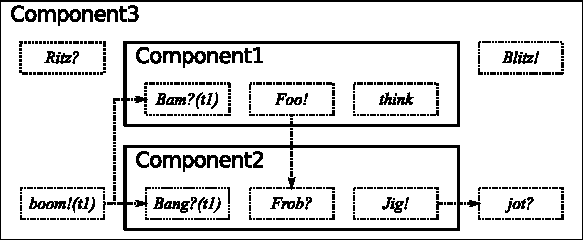
\includegraphics[width=\textwidth]{system_model}
\caption{Example event detection system.
  Automata are depicted as solid rectangles, e.g., Processor.
  Named automata are labeled by a box in their upper left corner, e.g., C.
  Actions are depicted as dotted rectangles, e.g., \emph{detect!}.
  Output actions are suffixed with \emph{!}, e.g., \emph{detect!}.
  Input actions are suffixed with \emph{?}, e.g., \emph{detected?}.
  Internal actions have no suffix, e.g., \emph{process1}.
  The type associated with a valued action is in parentheses after the name, e.g., \emph{out!(s)}.
  Bindings are indicate by dotted lines with an arrow pointing to the input.}
\label{sys_model}
\end{figure}

As a mathematical abstraction the I/O automata model is appropriate for modeling reactive asynchronous and concurrent systems.
However, it lacks certain features needed to develop real components.
This subsection introduces these features and lays the foundation for the dynamics discussed in section~\ref{dynamics}.

\paragraph{Recursive Encapsulation.}
Component frameworks that support recursive encapsulation allow components to contain other components.
Recursive encapsulation encodes the idea of ``divide-and-conquer'' and is at the heart of both bottom-up and top-down design strategies.
The contained component is the \emph{child} while the containing component is the \emph{parent}.
The resulting hierarchy helps developers organize programs by separating concerns and facilitates the reuse of existing components.
Distinction is made between the \emph{name} given to an instance and the \emph{type} of a child component to allow a parent component to contain multiple child of the same type.

For I/O automata, recursive encapsulation means that an I/O automaton can contain and use other I/O automata.
Recursive encapsulation implies that a parent automaton is the composition of itself and its children.
The \emph{root automaton} is the automaton at the top of the hierarchy and represents the entire system as composition is applied recursively to it and its children.
The sample event detector system of figure~\ref{sys_model} contains three automata (components):  an anonymous Processor, a Converter named C, and a Detector named D.
The Processor automaton is the root and C and D are its children.

\paragraph{Explicit Composition.}
Composition in the I/O automata model is based on actions having the same name and can be applied to an arbitrary number of automata.
Using recursive encapsulation, developers must have the ability to compose automata regardless of the naming convention used by the original developers.
To prepare for dynamic composition, we limit the scope of composition to associating a single output action with a single input action.
Such an association is called a \emph{binding} and is a pair $(output, input)$ where $output$ is the name of the output action and $input$ is the name of the input action.

Each automaton contains a set of bindings referring to its own actions, the actions of its children, the actions of its children's children, etc.
The automaton that prescribes a bindings is said to \emph{own} that binding.
The global set of bindings can be used to rename input actions before applying composition as defined by the I/O automata model.
A map for renaming inputs is generated by replacing action names with their fully-qualified name in all bindings by tracing from the root.
For the example in figure~\ref{sys_model}, this map is $\{ (out!(s), C.in?(s)), (C.out!(t), D.in?(t)), (D.detect!, detected?) \}$.
Composition as defined by the I/O automata model can be applied after using the map to rename all input actions to their corresponding output action.

\paragraph{Binding rules.}
To be compliant with the named-based composition of the I/O automata model, the set of bindings must adhere to certain rules.
First, the output action and input action of a binding must agree on the type being produced and consumed.
For example, an input action consuming an integer value can only be bound to an output action that produces an integer value.
The system in figure~\ref{sys_model} follows this rule since $(out!(s), C.in?(s))$ agree on type $s$, $(C.out!(t), D.in?(t))$ agree on type $t$, and $(D.detect!, detected?)$ agree on the absence of a value, i.e., a signal.
Second, an input action can be bound to at most one output action.
Composing an input action with multiple output actions would introduce ambiguity into the relationship between the states of the automata and is therefore prohibited by the model.
A binding map where all bindings that mention the same input action are equivalent satisfies this rule.
For dynamics, however, we strengthen this rule to say that an input action can appear at most once in the global binding map.
Consequently, every binding has exactly one owner.
Third, an output action cannot be bound to more than one input action in the same automaton.
This was rejected in the I/O automata model since the state of the automaton containing the input actions is not well-defined after the output is executed since the input action affects will be applied in undefined order.
Let $\pi$ be a prefix operator that strips the action name (leaving the path and hence the automaton) of a fully-qualified action name.
The following must be true for the global binding map $B$:  $\langle \forall o : (o, z) \in B :: \langle \forall i,j : (o, i) \in B \land (o, j) \in B \land i \neq j:: \pi (i) \neq \pi (j) \rangle \rangle$.
Fourth, an output action cannot be bound to an input action in the same automaton.
The I/O automata model prevents this by requiring that all actions belonging to the same automaton have a unique name.
Allowing such bindings result in undefined behavior since the order of the output and input effects is undefined.
To elaborate, we usually think about the output action occurring before the input action because a value must be generated.
However, the I/O automata model admits an interpretation where the value is generated first and the effects of the output action and input action are applied non-deterministically.
To adhere to this rule, the following must be true for the global binding map $B$:  $\langle \forall o, i : (o, i) \in B :: \pi (o) \neq \pi (i) \rangle$.

\paragraph{Concurrent execution.}
Recall that composing I/O automata consists of concatenating state vectors and folding input actions into output actions and that the result of composition is a single equivalent automaton.
Since the state of each automaton is independent, opportunities exist for the concurrent execution if the state of each automaton is preserved and a composition is not reduced to a single equivalent automaton.
Each local action implies a set of automata which in turn implies a set of state variables that might be modified.
For an internal action, this set consists of the automaton containing the internal action.
For an output action, this set consists of the automaton containing the output action and the automata that contain the input actions to which the output action is bound, i.e., composed.
Two actions can be executed concurrently if their respective sets of implied automata and therefore state variables are disjoint.
The implied automata sets for each local action in figure~\ref{sys_model} are: $out!(s) \to \{root, C\}$, $out!(t) \to \{C, D\}$, $process1 \to \{D\}$, $process2 \to \{D\}$, and $detect! \to \{D, root\}$.
Thus, $process1$ and $out!(s)$ can be executed concurrently while $process1$ and $detect!$ can not.

These observations create some interesting opportunities for designing and analyzing concurrent software.
Migrating intense computation to internal actions increases the level of parallelism in a system, i.e., the set of implied automata is small.
High degrees of fan-out, an output action being bound to many input actions, creates a bottle-neck and decreases the level of parallelism, i.e., the set of implied automata is large.
However, the input effects can be applied in parallel since the state of each automaton is independent.
High degrees of fan-in, an automaton has many bound input actions, also creates a bottle-neck by increasing the probability that two sets of implied automata will not be disjoint.
An high-performance scheduler might cluster and pin automata to processors to maximize concurrent execution while minimizing inter-processor communication.
A slow composition of automata might be statically composed to take advantage of in-lining.
A slow automaton might be factored into a number of child automata to increase parallelism.

\paragraph{Parameters.}
Actions in the I/O automata model can defined using parameters.
Parameters are useful for situations requiring fan-in or a session.
For example, consider an automaton with an input actions $in?(s)$ that is to be bound to $N$ different output actions.
The solution is to parameterize the input action with a parameter that indicates the associated output actions, e.g., $in?[i](s)$ where $i$ takes on the integer values from 1 to $N$.
\emph{Parameterized} actions take a parameter while \emph{unparameterized} actions do not.
Parameters, for actions that require them, are specified in the binding and serve to identify the action.

\paragraph{Action types.}
The combination of input, output, and internal actions, unvalued and valued, unparameterized and parameterized results in 10 possible action types:
unvalued unparameterized output (uv-up output),
unvalued parameterized output (uv-p output),
valued unparameterized output (v-up output),
valued parameterized output (v-p output),
unvalued unparameterized input (uv-up input),
unvalued parameterized input (uv-p input),
valued unparameterized input (v-up input),
valued parameterized input (v-p input),
unparameterized internal (up internal), and
parameterized internal (p internal).

\begin{figure}
\center
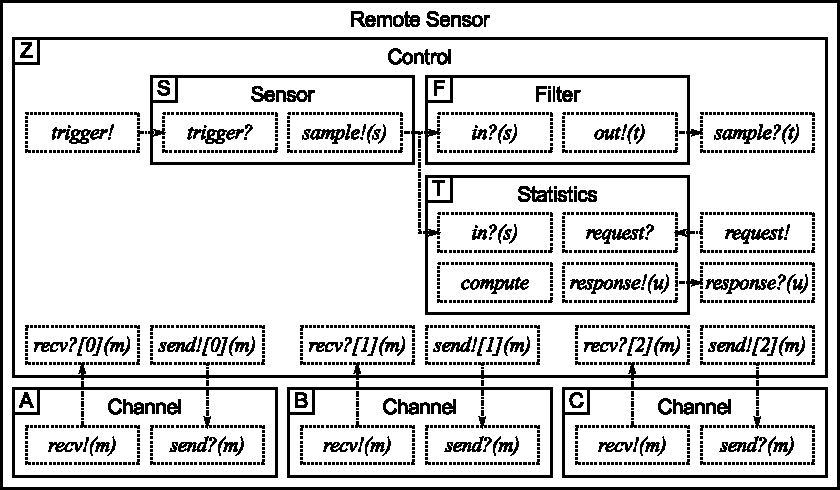
\includegraphics[width=\textwidth]{example1}
\caption{Example remote sensor system.
  Automata are depicted as solid rectangles, e.g., Remote Sensor.
  Named automata are labeled by a box in their upper left corner, e.g., Z.
  Actions are depicted as dotted rectangles, e.g., \emph{trigger!}.
  Output actions are suffixed with \emph{!}, e.g., \emph{trigger!}.
  Input actions are suffixed with \emph{?}, e.g., \emph{trigger?}.
  Internal actions have no suffix, e.g., \emph{compute}.
  The type associated with a valued action is in parentheses after the name, e.g., \emph{in?(s)}.
  Parameters are given in brackets after the action name, e.g., \emph{recv?[0](m)}.
  Bindings are indicate by dotted lines with an arrow pointing to the input.
}
\label{example1}
\end{figure}

\paragraph{Example.}
Figure~\ref{example1} depicts a remote sensor systems as a composition of automata.
The Remote Sensor automaton consists of the Control automaton $Z$ and three Channel automata $A$, $B$, and $C$ representing three network connections.
The Control automaton $Z$ consists of the Sensor automaton $S$, the Filter automaton $F$, and the Statistics automaton $T$.
The Control automaton $C$ starts the sampling process with the uv-up output $Z.trigger!$.
The uv-up input $S.trigger?$ is executed atomically with $Z.trigger!$ due to the binding $(Z.trigger!, S.trigger?)$.
When the sampling process is complete, the v-up output $S.sample!(s)$ distributes the sample to the Filter $F$ and Statistics component $T$ via the $(S.sample!(s), F.in?(s))$ and $(S.sample!(s), T.in?(s))$ bindings.
Note that $S.sample!(s)$, $F.in?(s)$, and $T.in?(s)$ all agree on the type of the sample $s$.
The Filter automaton $F$ passes the filtered sample to the Control automaton $Z$ via the $F.out!(t) \to Z.sample?(t)$ binding.
The Statistics automaton $T$ calculates the statistics incrementally using the up internal $T.compute$.
The statistics can be polled by the Control automaton $Z$ using the bindings $(Z.request!, T.request?)$ and $(T.response!(u), Z.response?(u))$.
The Control automaton $Z$ contains a vp-output $Z.send![](m)$ and a vp-input $Z.recv?[](m)$ for sending and receiving network messages using the Channel automata $A$, $B$, and $C$.
The parameters 0, 1, and 2, are used to route messages to Channel automata $A$, $B$, and $C$ respectively using the session idea mentioned previously.
Opportunities for concurrent execution exist for the remote sensor depicted in figure~\ref{example1}.
The set of automata implied by $Z.trigger!$ is $\{Z, S\}$ while the set of automata implied by $T.compute$ is $\{T\}$.
Since the sets are disjoint, the two actions can be executed concurrently.
